% Options for packages loaded elsewhere
\PassOptionsToPackage{unicode}{hyperref}
\PassOptionsToPackage{hyphens}{url}
\documentclass[
]{article}
\usepackage{xcolor}
\usepackage{amsmath,amssymb}
\setcounter{secnumdepth}{-\maxdimen} % remove section numbering
\usepackage{iftex}
\ifPDFTeX
  \usepackage[T1]{fontenc}
  \usepackage[utf8]{inputenc}
  \usepackage{textcomp} % provide euro and other symbols
\else % if luatex or xetex
  \usepackage{unicode-math} % this also loads fontspec
  \defaultfontfeatures{Scale=MatchLowercase}
  \defaultfontfeatures[\rmfamily]{Ligatures=TeX,Scale=1}
\fi
\usepackage{lmodern}
\ifPDFTeX\else
  % xetex/luatex font selection
\fi
% Use upquote if available, for straight quotes in verbatim environments
\IfFileExists{upquote.sty}{\usepackage{upquote}}{}
\IfFileExists{microtype.sty}{% use microtype if available
  \usepackage[]{microtype}
  \UseMicrotypeSet[protrusion]{basicmath} % disable protrusion for tt fonts
}{}
\makeatletter
\@ifundefined{KOMAClassName}{% if non-KOMA class
  \IfFileExists{parskip.sty}{%
    \usepackage{parskip}
  }{% else
    \setlength{\parindent}{0pt}
    \setlength{\parskip}{6pt plus 2pt minus 1pt}}
}{% if KOMA class
  \KOMAoptions{parskip=half}}
\makeatother
\usepackage{graphicx}
\makeatletter
\newsavebox\pandoc@box
\newcommand*\pandocbounded[1]{% scales image to fit in text height/width
  \sbox\pandoc@box{#1}%
  \Gscale@div\@tempa{\textheight}{\dimexpr\ht\pandoc@box+\dp\pandoc@box\relax}%
  \Gscale@div\@tempb{\linewidth}{\wd\pandoc@box}%
  \ifdim\@tempb\p@<\@tempa\p@\let\@tempa\@tempb\fi% select the smaller of both
  \ifdim\@tempa\p@<\p@\scalebox{\@tempa}{\usebox\pandoc@box}%
  \else\usebox{\pandoc@box}%
  \fi%
}
% Set default figure placement to htbp
\def\fps@figure{htbp}
\makeatother
\setlength{\emergencystretch}{3em} % prevent overfull lines
\providecommand{\tightlist}{%
  \setlength{\itemsep}{0pt}\setlength{\parskip}{0pt}}
\usepackage{bookmark}
\IfFileExists{xurl.sty}{\usepackage{xurl}}{} % add URL line breaks if available
\urlstyle{same}
\hypersetup{
  hidelinks,
  pdfcreator={LaTeX via pandoc}}

\author{}
\date{}

\begin{document}

Paul Koop


\includegraphics[width=4.92849in,height=4.92031in]{media/image6.png}

I.R.A.R.A.H. antwortet

Die Fortsetzung von Das Pompeji Projekt IRAHRA

Eine weitere Kurzgeschichte zum Posthumanismus

Das Team um Martina, Michael, Julia und Michaels Doppelgänger wird von
I.R.A.R.A.H. gerettet und muss vor dem Beginn eines neuen Lebens in
Budapest einige Abenteuer in Deutschland, in den USA und an der
ukrainisch-rumänischen Grenze überstehen. In Budapest treffen Michael
und sein Doppelgänger aufeinander.

Inhaltsverzeichnis

\hyperref[spurlos-verschwunden]{\textbf{Spurlos verschwunden 2}}

\hyperref[eingekleidet-in-der-wahrheit]{\textbf{Eingekleidet in der
Wahrheit 18}}

\hyperref[flucht-uxfcber-die-theiuxdf]{\textbf{Flucht über die Theiß
23}}

\hyperref[wiedersehen-in-budapest]{\textbf{Wiedersehen in Budapest 29}}

\section{Spurlos verschwunden}\label{spurlos-verschwunden}


\includegraphics[width=4.11458in,height=4.09375in]{media/image2.png}

Der Regen fiel in sanften, gleichmäßigen Tropfen auf die
Ausgrabungsstätte im Archäologischen Park von Pompeji. Die Erde unter
den Füßen der Archäologen verwandelte sich allmählich in eine zähe,
schlammige Masse, während das rhythmische Plätschern des Wassers die
einzigen Geräusche waren, die die Stille durchbrachen. Über den Ruinen
hingen dichte, graue Wolken, so tief, dass sie die umgebenden Hügel zu
verschlucken schienen. Die Welt wirkte wie in einen feuchten Schleier
gehüllt, und die antiken Mauern und ausgegrabenen Relikte erschienen
noch vergänglicher, als ob sie jeden Moment wieder im Boden verschwinden
könnten.

Dr. Leonardo Moretti, der Leiter der Ausgrabungen, stand über eine
brüchige Steinmauer gelehnt, seine grauen Augen fixierten den
Fortschritt der Arbeiten. Sein wettergegerbtes Gesicht war ernst, und
seine Gedanken wanderten zurück in die Jahrhunderte, als diese Straßen
und Gebäude noch von den Bewohnern Pompejis belebt gewesen waren. Die
vergangenen Tage hatten vielversprechende Funde zutage gebracht --
Fragmente von Inschriften und gut erhaltene Haushaltsgegenstände, die
den Alltag der alten Römer offenbarten. Doch heute lag eine
eigentümliche Unruhe in der Luft, die sich nicht allein durch das Wetter
erklären ließ.

Plötzlich kam ein Assistent hastig auf ihn zu, die durchnässte Kleidung
klebte an seinem schmalen Körper, und der Schlamm spritzte bei jedem
Schritt auf. „Dr. Moretti, die Inschrift ist fast freigelegt. Wir
brauchen Martina Rossi für die Begutachtung``, sagte der junge Mann,
seine Stimme klang leise, aber besorgt.

Moretti blickte von der Mauer auf und zog die Stirn kraus. Martina war
die Expertin für antike Schriften, sie wurde stets herbeigerufen, sobald
eine neue Inschrift sichtbar wurde. „Wo ist sie? Sie sollte längst hier
sein``, erwiderte er, seine Stimme schärfer als beabsichtigt.

Der Assistent zuckte mit den Schultern, und ein nervöses Zucken lief
über sein Gesicht. „Keiner hat sie heute gesehen. Sie war auch nicht
beim Frühstück``, antwortete er und wich Morettis Blick aus.

Ein seltsames Gefühl kroch in Moretti hoch, als ob sich eine unsichtbare
Hand um seinen Magen legte und ihn langsam zusammenpresste. Martina war
zuverlässig, eine Frau, die jede Verabredung und jede Aufgabe ernst
nahm. Dass sie einfach nicht erschien, ohne Bescheid zu geben, war
ungewöhnlich -- zu ungewöhnlich, um es zu ignorieren. Er sah auf seine
Uhr. Es war schon fast Mittag. Der Regen prasselte weiter in
gleichmäßigen Tropfen auf den Steinboden, und die Dunkelheit der Wolken
hatte etwas Bedrückendes.

„Ich gehe nach ihr sehen``, sagte Moretti schließlich, mehr zu sich
selbst als zu seinem Assistenten, und ließ den Blick über die
Ausgrabungsstätte schweifen. Seine Gedanken rasten bereits, während er
den Arbeitsbereich verließ. Er konnte die Schritte der anderen
Archäologen auf dem nassen Stein kaum noch hören, als er sich vom Lärm
der Arbeit entfernte. Die Mauerreste und Trümmer schienen wie stumme
Zeugen seines wachsenden Unbehagens über ihm zu thronen.

Moretti eilte zu seinem Auto, das am Rand der Ausgrabungsstätte geparkt
war. Er drehte sich kurz um und sah, wie die Arbeiter unter den
schützenden Planen weitermachten, unbeeindruckt vom Regen, der jetzt
nachzulassen schien. Ein leichter Wind hob die schweren Wolken ein Stück
an, sodass der Himmel aufriss und ein wenig Licht hindurchließ. In
seiner Eile vergaß Moretti seinen Regenschirm an einem der Tische auf
dem Gelände -- ein dummer Fehler, wie ihm nun bewusst wurde. Als er den
kurzen Weg zu seinem Auto zurücklegte, bemerkte er, dass die Tropfen von
den Blättern der Bäume auf seinen Kragen plätscherten und seine Kleidung
feucht machten. Die Kälte kroch durch den Stoff hindurch und ließ ihn
leicht zittern.

Im Wageninneren ließ er den Motor aufheulen und setzte den
Scheibenwischer in Bewegung. Das leise Kratzen des Wischers über die
Windschutzscheibe mischte sich mit dem beständigen Ticken der Uhr im
Armaturenbrett, das ihm auf unerklärliche Weise unheimlich erschien.
Moretti spürte, wie sich die Anspannung in seinen Schultern festsetzte.
Er dachte an Martina und auch an Julia, ihre Freundin und Mitbewohnerin.
Beide waren wie Schwestern, die unzertrennlich schienen, auch abseits
der Arbeit.

Was war geschehen? Sein Kopf war voller Gedanken, die sich in
chaotischen Bahnen bewegten, und je mehr er darüber nachdachte, desto
unruhiger wurde er. Hatten sie sich verletzt? Gab es einen Unfall? Er
verwarf den Gedanken. Es wäre ihm doch zu Ohren gekommen, wenn etwas
passiert wäre.

Er warf einen letzten Blick auf das Gelände, bevor er in die schmale,
regennasse Straße einbog, die zu der Wohnung von Martina und Julia
führte. Die Scheibenwischer glitten unermüdlich über das Glas, als er
das Gaspedal durchdrückte.

Vor dem kleinen italienischen Wohnhaus, dessen Fassade sich in warmem
Ocker und bröckelndem Putz präsentierte, hielt Moretti an. Es war ein
vertrauter Anblick -- ein unscheinbares Gebäude in einer ruhigen
Seitenstraße von Pompeji, das er schon oft besucht hatte. Doch an diesem
regnerischen Tag wirkte es anders, als ob sich eine unsichtbare
Bedrohung über den Ort gelegt hätte. Die Fensterläden klapperten leise
im Wind, und der Regen tropfte von den Dachkanten herab, als er aus dem
Auto stieg. Ein ungutes Gefühl wuchs in seiner Brust, als er sich dem
Eingang näherte, seine Schritte hallten dumpf auf dem nassen Pflaster
wider.

Moretti zögerte einen Augenblick vor der Tür von Martina und Julias
Wohnung, bevor er entschlossen klopfte. Seine Hand zitterte leicht, als
er die Faust gegen das dunkle Holz drückte. Er lauschte in die Stille,
hoffte, dass jeden Moment Schritte zu hören wären, dass eine der Frauen
die Tür öffnen und ihn mit einem entschuldigenden Lächeln begrüßen
würde. Doch es blieb still. Er klopfte erneut, diesmal etwas lauter, die
Anspannung ließ seine Stimme in seinem Kopf lauter widerhallen als die
Schläge auf das Holz. Aber auch jetzt blieb alles ruhig -- kein Geräusch
aus dem Inneren der Wohnung, keine Antwort.

Ein Gefühl der Besorgnis durchfuhr ihn, wie ein kalter Windstoß, der
durch die halbgeöffneten Fensterläden wehte. Das passte nicht zu
Martina. Sie war immer organisiert, zuverlässig, die Art von Person, die
für jede Gelegenheit einen Plan hatte. Moretti warf einen prüfenden
Blick zur Seite und entdeckte ein Fenster, das leicht geöffnet war. Er
trat näher, das leise Rauschen des Regens und das entfernte Summen der
Stadt hinter ihm verschwand in den Hintergrund, als seine Aufmerksamkeit
sich vollständig auf das Innere der Wohnung richtete.

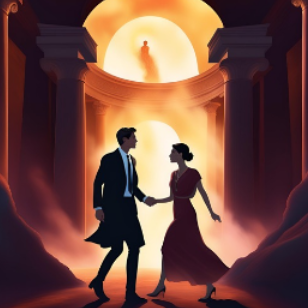
\includegraphics[width=4.14583in,height=4.11458in]{media/image8.png}

Er spähte durch den Spalt des Fensters, und was er sah, ließ sein Herz
schneller schlagen. Das Innere der Wohnung war ein einziges Chaos --
Kleidung lag verstreut auf den Betten, als ob sie hastig durchwühlt
worden wären. Ein halbgepackter Koffer stand im Flur, schief und
geöffnet, als hätte jemand ihn in der Eile stehen lassen. Papiere und
Notizen waren auf dem Küchentisch verteilt, als ob jemand auf der Suche
nach etwas Wichtigem gewesen wäre. Die Szenerie hatte etwas
Unwirkliches, fast wie ein gestelltes Bild, doch die Unordnung sprach
Bände über eine plötzliche und unvorbereitete Abreise.

Moretti zog sich vom Fenster zurück, sein Herz hämmerte in seiner Brust,
als die Realität der Situation ihm klar wurde. „Das passt nicht zu
Martina. Sie ist immer so ordentlich``, dachte er, während sich die
Besorgnis zu einem regelrechten Druck auf seiner Brust verdichtete. Eine
Unruhe ergriff ihn, die er nicht mehr abstreifen konnte. Die Szene im
Inneren des Hauses jagte ihm einen Schauer über den Rücken, als er sich
fragte, was geschehen sein könnte.

Seine Gedanken überschlugen sich: Hatten sie einfach in Panik alles
liegen und stehen lassen? War es ein Unfall oder etwas anderes, etwas
Dunkleres, das sie zum Verschwinden gezwungen hatte? Er konnte sich
keinen Reim darauf machen, doch eines war klar: Das hier war mehr als
nur ein Missverständnis oder ein Versehen.

Die Ungeduld stieg in ihm auf wie das kalte Regenwasser, das sich an
seinen Schuhen sammelte. Moretti wandte sich abrupt von der Tür ab, lief
mit schnellen Schritten zurück zu seinem Auto. Das Gefühl der
Dringlichkeit nagte nun unerbittlich an ihm, wie ein bohrender Schmerz,
der immer heftiger wurde. Ohne lange zu überlegen, sprang er ins Auto,
ließ den Motor aufheulen und fuhr mit durchdrehenden Reifen los. Das
Wasser spritzte von den Straßenrändern auf, als er in die nasse, schmale
Straße einbog, die zur nächsten Polizeistation führte. Sein Kopf war
voller Fragen, aber nur eine Sache war jetzt von Bedeutung: Er musste
Hilfe holen, und das so schnell wie möglich.

Es war ein grauer, verregneter Vormittag, als Dr. Leonardo Moretti durch
die schweren Glastüren der Polizeistation in Neapel trat. Der feuchte
Geruch der Stadt haftete an seiner Kleidung, und seine nassen Schuhe
quietschten leise auf dem kühlen Marmorboden. Die Wolken hingen tief und
düster über der Stadt, als drückten sie das Leben und die Hektik Neapels
nieder, die man durch die offenen Fenster hindurch hören konnte --
hupende Autos, rufende Straßenhändler und das leise, gleichmäßige
Rauschen des Regens.

Moretti, dessen Gesicht von der Sonne vergangener Ausgrabungen gegerbt
war und dessen Haare an den Schläfen bereits ergraut waren, fühlte einen
Kloß in seinem Hals. Die Unruhe, die ihn seit dem Morgen begleitete,
hatte sich zu einer beängstigenden Gewissheit verdichtet. Er ging
schnellen Schrittes auf den Tresen des Empfangs zu, wo ein junger
Polizist hinter einem Haufen von Akten saß. Die Schritte des Archäologen
hallten durch den Raum, jeder Schritt ein Echo der drängenden Sorge, die
ihn hierhergetrieben hatte.

„Ich möchte eine Vermisstenanzeige aufgeben``, sagte Moretti, seine
Stimme drängte und klang zugleich erschöpft. Er bemühte sich, Ruhe zu
bewahren, doch ein Hauch von Dringlichkeit schwang unweigerlich in
seinen Worten mit. „Zwei meiner Kollegen -- Historikerin Martina Rossi
und ihre Mutter Julia Rossi -- sind seit gestern Abend verschwunden. Sie
sollten heute Morgen bei den Ausgrabungen sein. Ihre Wohnung...`` Er
hielt kurz inne, als würde er nach den richtigen Worten suchen. „Es ist
ein Chaos, als ob sie in Eile waren.``

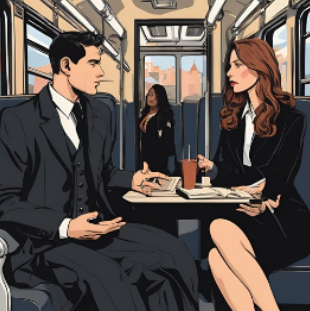
\includegraphics[width=4.0625in,height=5.61458in]{media/image3.png}

Der Polizist hob den Blick von den Papieren auf seinem Schreibtisch und
musterte Moretti mit einem prüfenden Blick, dann griff er gemächlich
nach einem Notizblock und einem Stift. „Wann haben Sie die beiden
zuletzt gesehen?{\kern0pt}`` fragte er sachlich, während er sich langsam
für das Protokoll bereit machte.

„Gestern Nachmittag, bei der Arbeit``, antwortete Moretti rasch. „Sie
waren wie immer in der Nähe der neuen Ausgrabungsstelle. Es gab nichts
Ungewöhnliches, keine Anzeichen dafür, dass irgendetwas nicht stimmte.
Aber danach habe ich nichts mehr von ihnen gehört. Sie sind
einfach\ldots{} verschwunden.`` Morettis Stimme brach leicht, ein
seltenes Zittern in seinen Worten, das er nicht unterdrücken konnte.

Der Polizist nickte, begann die Angaben niederzuschreiben und zog
abermals seine Augenbrauen zusammen, während er die Details notierte.
„Sie sagen, ihre Wohnung sei in Unordnung gewesen?{\kern0pt}`` fragte er
mit einem leichten Stirnrunzeln. „Gab es Anzeichen von Gewalt oder einem
Kampf?{\kern0pt}``

Moretti schüttelte den Kopf. „Nein, nichts dergleichen. Aber es war
nicht normal... die Koffer waren halb gepackt, Kleidung war überall
verteilt, als ob sie überstürzt aufbrechen wollten.``

Der Polizist ließ den Stift einen Augenblick ruhen und sah Moretti an,
als ob er versuchte, die Bedeutung hinter den Worten des Archäologen zu
ergründen. „Wir werden die Anzeige aufnehmen und sofort mit den
Ermittlungen beginnen``, sagte er schließlich mit einem Tonfall, der
wohl beruhigend wirken sollte, aber an Morettis nagender Sorge wenig
ändern konnte.

„Danke``, erwiderte Moretti und nickte kurz, doch seine Gedanken waren
bereits bei den nächsten Schritten. Was war mit Martina und Julia
geschehen? Jede Sekunde fühlte sich an, als ob sie mit tausend Fragen
gefüllt wäre, auf die er keine Antwort hatte. Während der Polizist
begann, in die Tiefen der Bürokratie einzutauchen, um die ersten
Maßnahmen einzuleiten, fühlte Moretti die Kälte des Marmorbodens durch
seine nassen Schuhe kriechen, als würde die Stadt selbst ihre düstere
Stimmung in sein Herz übertragen.

Er trat einen Schritt zurück und sah sich in der Station um -- Beamte
eilten an ihm vorbei, Telefone klingelten, und das Murmeln von
Gesprächen mischte sich mit den Geräuschen der Stadt, die durch die
Fenster hereinströmten. Moretti fühlte sich in diesem Moment seltsam
fehl am Platz. Hier, in der Welt der Ordnung und Vorschriften, konnte er
nur hoffen, dass die Unruhe in seiner Brust bald einer Antwort weichen
würde. Doch als er die Polizei verlassen wollte, wusste er tief in
seinem Inneren, dass dies erst der Anfang war -- die ersten Schritte in
ein düsteres Labyrinth, in dem das Verschwinden seiner Kolleginnen
möglicherweise mehr Fragen aufwerfen würde, als er sich je hätte
vorstellen können.

Die Polizei nahm den Fall von Anfang an ernst. Es war mehr als nur ein
Routinevorgang -- es war das unbehagliche Gefühl, das selbst die
erfahrensten Beamten nicht ignorieren konnten, wenn zwei Menschen
plötzlich und ohne jede Spur verschwanden. Der Polizist am Empfang, der
Morettis Vermisstenanzeige aufgenommen hatte, übergab die Akte mit einem
knappen Nicken an zwei Ermittler, die auf solche Fälle spezialisiert
waren. Ein Hauch von Dringlichkeit lag in der Luft, als die beiden
Beamten, ein älterer Mann mit grau meliertem Haar und sein jüngerer
Kollege mit entschlossener Miene, die Akte durchblätterten.

Im Büro herrschte hektische Betriebsamkeit. Das Klappern von
Computertasten mischte sich mit dem Gemurmel der Polizisten und den
Anrufen auf den Telefonleitungen, während die Ermittler die Details des
Falls durchgingen. „Zwei Frauen, Mutter und Tochter, seit gestern Abend
vermisst``, las der Ältere laut vor. „Wohnung im Chaos, keine Anzeichen
eines Kampfes.`` Er tauschte einen bedeutungsvollen Blick mit seinem
Kollegen aus, bevor er entschlossen die Autotür seines Dienstwagens
aufschwang.

Nur wenige Minuten später saßen die beiden Ermittler bereits im Auto und
fuhren durch die regennassen Straßen Neapels in Richtung Pompeji. Der
Himmel war weiterhin von schweren Wolken bedeckt, und der Nieselregen
setzte sich auf der Windschutzscheibe ab, während der Scheibenwischer
monoton hin und her schwang. Die Fahrt war kurz, doch in dieser kurzen
Zeit malte sich in den Köpfen der beiden Polizisten bereits ein Bild der
Möglichkeiten aus. Es war ihre Aufgabe, alle Szenarien zu durchdenken --
und in dieser Gegend, in der die Schatten der Camorra allgegenwärtig
waren, konnte es viele Gründe geben, warum zwei Frauen spurlos
verschwunden waren.

Als sie das Wohnhaus erreichten, stieg der ältere Ermittler aus und zog
seinen Mantel enger um sich. Die Tür der Wohnung stand einen Spalt weit
offen, ein Detail, das sofort seine Aufmerksamkeit auf sich zog. „Das
ist nicht gut``, murmelte er, und sein jüngerer Kollege nickte, während
er mit einem geübten Griff seine Handschuhe aus der Tasche zog. Sie
betraten die Wohnung vorsichtig, die Luft war abgestanden und kalt. Das
Licht war schwach, und die Stille, die im Raum hing, war unnatürlich.

Kleidung war über die Betten verteilt, als wären sie in aller Eile
zurückgelassen worden. Ein halbgepackter Koffer stand im Flur, der
Deckel offen, und ein Schuh lag einsam auf dem Boden, während sein Paar
nirgendwo zu sehen war. Auf dem Küchentisch lagen offene Briefe und
Notizen, einige davon zerknittert, als hätte jemand sie hastig
weggeworfen. Der Jüngere bückte sich und hob eine der Notizen auf. „Es
sieht aus, als ob sie mitten in den Vorbereitungen für eine Reise
waren``, sagte er leise und ließ den Zettel wieder zurück auf den Tisch
fallen.

„Das sieht nach einem hastigen Aufbruch aus``, murmelte der ältere
Ermittler und ließ seinen Blick durch den Raum schweifen. „Kleidung
liegt herum, die Koffer sind nicht fertig gepackt. Aber es gibt keine
Anzeichen eines Kampfes.`` Er ging einige Schritte weiter, öffnete eine
Tür, die ins Badezimmer führte, und fand auch dort nichts Auffälliges.
Alles war auf den ersten Blick normal, bis auf die Unordnung -- ein
unerwartetes Durcheinander in einer sonst ordentlichen Wohnung.

Der jüngere Ermittler trat an eines der Fenster und zog die Jalousien
hoch, um besser sehen zu können. Das Tageslicht, wenn auch grau und
trüb, fiel in den Raum und beleuchtete die Details der Unordnung noch
deutlicher. „Vielleicht sind sie geflüchtet oder wollten unbemerkt
abreisen``, sagte er nachdenklich. „Es gibt keinen Hinweis darauf, dass
jemand sie mit Gewalt mitgenommen hat.`` Er ging auf die Knie und
untersuchte die Spuren auf dem Boden, fand aber nichts, was auf einen
Kampf oder ein Verbrechen hindeutete.

Zurück auf der Polizeistation in Neapel herrschte eine gespannte
Atmosphäre. Die beiden Ermittler versammelten sich mit weiteren Kollegen
in einem Besprechungsraum, um die bisherigen Erkenntnisse
zusammenzutragen. Die Möglichkeit, dass es sich um einen gewöhnlichen
Vermisstenfall handelte, schwand zusehends. Es gab zu viele offene
Fragen, und die Tatsache, dass sich die Wohnung in einem solchen Zustand
befand, ließ ihnen keine Ruhe.

„Das Ganze spielt sich in einer Gegend ab, in der die Camorra ihre
Finger im Spiel hat``, bemerkte der ältere Ermittler und warf einen
skeptischen Blick auf die Karte, die an der Wand hing. „Es wäre nicht
das erste Mal, dass Menschen spurlos verschwinden, wenn sie sich
ungewollt in die Machenschaften der lokalen Kriminalität einmischen.``
Sein Kollege nickte zustimmend. Es war keine seltene Geschichte, dass
jemand zur falschen Zeit am falschen Ort war und dann nicht mehr gesehen
wurde.

Es war klar, dass dieser Fall über die Zuständigkeit der normalen
Ermittlungen hinausging. Die Entscheidung, den Fall an die
Staatsanwaltschaft zu übergeben, fiel schnell, und damit wurde auch die
Direzione Distrettuale Antimafia, die für organisierte Kriminalität
zuständig war, einbezogen. Zu viele Fragen blieben unbeantwortet, und
der Gedanke, dass mehr hinter dem Verschwinden der Frauen stecken
könnte, ließ die Ermittler nicht los.

Während die Beamten in der Polizeistation hektisch weiterarbeiteten, um
die ersten Spuren zu sichern und Zeugen zu befragen, breitete sich das
unbehagliche Gefühl aus, dass sie es mit einem Fall zu tun hatten, der
dunkler und gefährlicher war, als es auf den ersten Blick erschien.

Im Büro der Staatsanwaltschaft herrschte eine bedrückende Stille, als
der Staatsanwalt, ein Mann mittleren Alters mit tiefen Falten um die
Augen und einem Stirnrunzeln, das jahrelanger Schlafmangel geprägt
hatte, die ersten Berichte durchblätterte. Die Aktenberge vor ihm
schienen förmlich zu pulsieren, so dringlich war die Situation. „Ein
solcher Fall in der Nähe von Pompeji könnte durchaus mit der lokalen
Camorra in Verbindung stehen``, murmelte er, seine Stimme ruhig, aber
bestimmt. Er legte den Bericht mit einem dumpfen Geräusch auf den Tisch
und sah die versammelten Ermittler nacheinander an. „Wir müssen jede
Spur verfolgen -- Bankverbindungen, Telefonaktivitäten, Kontakte. Prüfen
Sie, ob sie kürzlich größere Beträge abgehoben oder auffällige Einkäufe
getätigt haben. Kein Detail ist zu unbedeutend.``

Die Ermittler standen angespannt da, die Luft im Raum schien schwerer zu
werden. Einer der jüngeren Beamten trat vor, sein Blick entschlossen.
„Ihre Arbeitsstelle hat die Vermisstenmeldung offiziell bestätigt. Die
Kollegen bei den Ausgrabungen sind äußerst besorgt. Ich schlage vor, wir
untersuchen auch dort noch einmal gründlich. Es könnte Hinweise geben,
die wir übersehen haben.``

Der Staatsanwalt nickte zustimmend. „Gut, tun Sie das. Und ich möchte,
dass die Direzione Distrettuale Antimafia (DDA) eingebunden wird. Wenn
die Camorra ihre Finger im Spiel hat, brauchen wir die besten Leute auf
diesem Fall.`` Er strich sich über sein unrasiertes Kinn und dachte
einen Moment nach. „Und halten Sie nach allem Ausschau, was mit
historischen Artefakten zusammenhängen könnte. In der Gegend gibt es
viele wertvolle Ausgrabungen, die das Interesse der organisierten
Kriminalität wecken könnten.``

Während die Ermittler ihre Anweisungen entgegennahmen, griffen sie
bereits zu ihren Handys, um erste Befragungen zu organisieren und die
nächsten Schritte einzuleiten. Sie wussten, dass sie unter großem Druck
standen -- nicht nur, weil zwei Menschen vermisst wurden, sondern auch,
weil es hier um mehr ging: um Macht, um Geschichte und vielleicht sogar
um Leben und Tod.

Unterdessen bereitete ARS, die Künstliche Intelligenz, die im Geheimen
für I.R.A.R.A.H operierte, ihre nächste digitale Täuschung vor. Es war,
als ob ARS bereits vorausgesehen hatte, dass die Behörden tiefer graben
würden. In den Netzwerken der Polizei und der Fluggesellschaften
arbeiteten ihre Algorithmen schnell und effizient. Flug- und
Reiseaufzeichnungen wurden manipuliert oder gelöscht, Buchungen
storniert und Passagierlisten gefälscht. Es sah jetzt so aus, als hätten
Martina und Julia niemals die Stadt verlassen. Die Künstliche
Intelligenz verschleierte die Spuren so gründlich, dass selbst erfahrene
Ermittler in einem Dickicht aus falschen Fährten und irreführenden
Informationen gefangen waren.

Doch die Behörden ließen sich nicht so leicht entmutigen. Der Verdacht,
dass die beiden Historikerinnen etwas entdeckt haben könnten, das nicht
ans Tageslicht kommen sollte, schien zu konkret, um ihn einfach abzutun.
Ein paar Tage später, nachdem die Ermittler die Ausgrabungsstätte erneut
untersucht und weitere Befragungen durchgeführt hatten, stießen sie auf
einen neuen Hinweis. Bei einer gründlichen Durchsuchung der Wohnung von
Martina und Julia fanden sie eine Visitenkarte -- Michael Phillips,
Professor an der Gregoriana in Rom.

Die Ermittler betrachteten die Karte nachdenklich. „Wer ist dieser Mann,
und warum hatten sie seine Visitenkarte?{\kern0pt}`` fragte einer der
Beamten laut. Die Tatsache, dass Michael Phillips in der Nähe des
Vatikans arbeitete, ließ sie aufhorchen. Es war eine Verbindung, die in
vielerlei Hinsicht Bedeutung haben konnte. Die Nähe zur religiösen und
akademischen Elite Roms, die Verbindungen in die intellektuelle Welt --
alles schien plötzlich wichtig.

Ein Anruf wurde getätigt, und kurz darauf wurde ein Team
zusammengestellt, das nach Rom geschickt werden sollte, um mit Michael
Phillips zu sprechen. Die Ermittler bereiteten ihre Fragen sorgfältig
vor, sammelten Informationen über den Professor und seine Arbeit, um ihm
während der Befragung keine Möglichkeit zu geben, sich herauszuwinden.

Währenddessen saß Michael Phillips in seinem Büro an der Gregoriana. Es
war ein warmer, stiller Raum, geschmückt mit Bücherregalen, die von der
Decke bis zum Boden reichten. Das Licht seiner Schreibtischlampe warf
lange Schatten auf den hölzernen Tisch. Er hatte das Gefühl, als würden
sich diese Schatten immer näher an ihn heranschieben. Seit Tagen spürte
er, wie die Anspannung um ihn herum wuchs, wie ein Netz, das sich
langsam, aber unaufhaltsam zusammenzog. Die Ermittlungen in Neapel
hatten an Fahrt aufgenommen, und er wusste, dass Martina und Julia nun
ins Zentrum der Aufmerksamkeit der Behörden rückten -- und damit auch
er.

Eine verschlüsselte Nachricht von ARS war kurz zuvor auf seinem Laptop
eingetroffen. „Die Eintragungen bei der Flugsicherung wurden erfolgreich
gelöscht. Keine weiteren Spuren in den Datenbanken``, las er auf dem
Bildschirm. Es war eine Art von Erleichterung, die durch seinen Körper
strömte, doch sie war flüchtig. Der Druck nahm nicht ab; im Gegenteil,
er wuchs mit jeder Minute, die verstrich, denn er wusste, dass der
kleinste Fehler alles gefährden könnte.

Als die Dämmerung über Rom hereinbrach, saß Michael weiterhin an seinem
Schreibtisch. Die Geräusche der Stadt drangen durch das offene Fenster:
das Summen der Straßenlaternen, die Motorengeräusche in der Ferne. Es
wirkte wie ein bedrückendes Crescendo, das seine Gedanken immer
schneller wirbeln ließ. Er wusste, dass die Ermittler bald ankommen
würden. Das Spiel hatte begonnen, und er musste sicherstellen, dass
I.R.A.R.A.H nicht aufflog. Es war ein riskantes Spiel -- eines, das mit
der Sicherheit von Martina und Julia auf dem Spiel stand.

Während er auf den Moment wartete, als es an seiner Bürotür klopfen
würde, lehnte sich Michael zurück und ließ seinen Blick über die
Buchrücken in den Regalen gleiten. Da waren Werke über Philosophie,
Theologie und Geschichte, doch jetzt schienen sie alle irrelevant zu
sein, angesichts dessen, was in den nächsten Stunden auf dem Spiel
stand.

Das Klopfen an der Tür ließ ihn zusammenzucken. Es war soweit. Die
Ermittler waren da, und Michael wusste, dass jedes Wort, das er gleich
sagen würde, mit Argusaugen beobachtet und analysiert werden würde.

Ein lautes Klopfen an der Tür durchbrach die Stille im Raum und ließ
Michael Phillips zusammenzucken. Er hatte diesen Moment erwartet,
vorbereitet darauf, die perfekte Maske aufzusetzen. Aber dennoch spürte
er das unbehagliche Ziehen in seinem Magen, das sich einfach nicht
vertreiben ließ. Mit einem tiefen Atemzug erhob er sich langsam, zwang
sich zur Ruhe, während er zur Tür ging und sie öffnete.

Zwei Männer in dunklen Anzügen standen vor ihm, der eine mit strengem,
unbeweglichem Gesichtsausdruck, während der andere seine Miene lockerer
hielt, doch in seinen Augen lag die kalte, zielgerichtete Schärfe eines
Jägers. „Dr. Phillips?{\kern0pt}`` sagte der erste mit einem Hauch von
Nachdruck in der Stimme. „Wir sind von der Polizia di Stato. Es geht um
eine Befragung zu dem Verschwinden von Martina Rossi und Julia Rossi.
Dürfen wir hereinkommen?{\kern0pt}``

Michael nickte stumm und trat zur Seite, um sie einzulassen. Die Männer
betraten sein Büro, und er konnte die verhaltene Spannung in ihren
Bewegungen spüren. Es war, als ob sie jede Falte in seinem Gesicht, jede
unwillkürliche Geste genau registrierten. Er führte sie zu einem
kleinen, runden Tisch in der Mitte des Raumes und setzte sich, während
die Ermittler ihre Plätze einnahmen. Der ernste Polizist nahm direkt vor
ihm Platz, fixierte ihn mit durchdringendem Blick, während der andere am
Rande des Raumes blieb, aufmerksam, jede Ecke des Büros mit den Augen
absuchend.

„Wir haben einige Fragen an Sie``, begann der Polizist und schlug sein
Notizbuch auf. „Sie kennen Martina Rossi und Julia Rossi sehr gut, nicht
wahr?{\kern0pt}`` Seine Stimme war ruhig, aber dahinter lag ein
unausgesprochenes Misstrauen.

„Ja``, antwortete Michael gelassen, seine Hände ruhend auf dem Tisch,
während er ihre Blicke erwiderte. „Ich habe mit ihnen an verschiedenen
Projekten gearbeitet, sowohl akademisch als auch im Rahmen von InSim.``

Der Polizist nickte knapp, als ob er es bereits gewusst hätte. „Martinas
Arbeitgeber hat eine Vermisstenanzeige erstattet. Sie wurde das letzte
Mal in Ihrer Nähe gesehen. Können Sie uns sagen, was am Tag ihres
Verschwindens geschah?{\kern0pt}``

Michael ließ sich einen Moment Zeit, bevor er antwortete, seine Gedanken
sorgsam sortierend, um keine ungewollten Hinweise zu geben. „Ich
erinnere mich, dass wir uns vor ihrer Abreise nach Pompeji getroffen
haben. Sie wollten zu einem Workshop zurück nach Italien. Alles schien
vollkommen normal.``

Die beiden Männer wechselten einen schnellen Blick, und der Polizist
lehnte sich leicht vor, als wollte er Michaels Gesichtsausdruck genauer
beobachten. „Normal?{\kern0pt}`` fragte er mit einem Hauch von Skepsis
in der Stimme. „Es gab keine Anzeichen, dass etwas nicht
stimmte?{\kern0pt}``

Michael schüttelte ruhig den Kopf, achtete darauf, nicht zu eifrig zu
wirken. „Nichts, was mir aufgefallen wäre``, erwiderte er gleichmütig.
Aber in seinem Inneren kämpfte er, das mulmige Gefühl zu verdrängen. In
diesem Moment summte das unsichtbare Interface von ARS leise in seinem
Ohr. Die Stimme der KI klang wie ein Flüstern aus einer anderen Welt:
„Sie überprüfen Flugzeugaufzeichnungen. Wir haben sie gelöscht. Bleib
ruhig.``

Der Ermittler fixierte ihn weiterhin mit seinem durchdringenden Blick.
„Und was wissen Sie über den Unfall des InSim-Mercedes, der in der Nähe
von Pompeji verunglückte? Zwei Zeugen behaupten, das Fahrzeug wurde von
einer unbekannten Gruppe verfolgt.``

Michael spürte, wie ihm ein leichter Schweißfilm auf die Stirn trat,
doch er zwang seine Miene, ruhig zu bleiben. ARS reagierte sofort und
schickte eine beruhigende Nachricht: „Wir haben die Überwachungsdaten
des Unfalls bearbeitet. Sie werden keine weiteren Beweise finden.``

„Mir ist nur bekannt, dass sie auf dem Weg zu einer Konferenz waren``,
sagte Michael mit so viel Gelassenheit, wie er aufbringen konnte. „Der
Unfall kam unerwartet. Ich war zu diesem Zeitpunkt in Rom.`` Er hoffte,
dass seine Stimme ruhig genug klang, auch wenn er innerlich spürte, wie
der Druck wuchs, jedes Detail perfekt abzuwägen.

Der Polizist beobachtete ihn noch einige Sekunden länger, als wollte er
etwas in seinen Augen erkennen, das Michael nicht preisgab. Dann griff
er in seine Jackentasche und zog eine Visitenkarte hervor, die er vor
Michael auf den Tisch legte. Die Karte wirkte klein und unscheinbar,
doch ihre Bedeutung war schwerwiegend. Es war Michaels eigene
Visitenkarte. „Diese Karte wurde bei den persönlichen Gegenständen der
Frauen gefunden``, erklärte der Ermittler ruhig. „Können Sie das
erklären?{\kern0pt}``

„Ja, das ist meine Karte``, antwortete Michael ohne zu zögern. „Ich habe
sie beiden gegeben, falls sie mich für akademische Fragen kontaktieren
wollten. Sie hatten in letzter Zeit viele technische Fragen, die sie
klären wollten.``

Ein tiefes Schweigen breitete sich im Raum aus, als ob die Luft selbst
schwerer geworden wäre. Michael spürte, wie sich die Spannung aufbaute,
spürte das Warten der Ermittler, als ob sie darauf lauerten, dass er
einen Fehler machte. Er hielt die Nerven, zwang sich, jede Spur von
Nervosität zu verbergen. Das sanfte Summen von ARS' Stimme blieb
konstant in seinem Ohr, ein ständiger, beruhigender Begleiter in diesem
gefährlichen Spiel.

Nach einer scheinbar endlosen Minute stand der zweite Ermittler auf und
ging zum Fenster. Er tat es beiläufig, aber Michael bemerkte die
Wachsamkeit in seinen Bewegungen, als ob er nach etwas suchte. „Sie
wissen nichts von ihrem jetzigen Aufenthaltsort?{\kern0pt}`` fragte er
über die Schulter hinweg. „Irgendwelche Hinweise, wo sie sein
könnten?{\kern0pt}``

„Leider nicht``, erwiderte Michael ruhig. „Ich mache mir auch Sorgen um
sie.``

Der zweite Ermittler kam zurück, beugte sich über den Tisch und fixierte
Michael mit einem durchdringenden Blick, der keine Zweifel zuließ.
„Sollten Sie uns etwas verheimlichen, Dr. Phillips, werden wir es
herausfinden. Das wissen Sie.``

Michael lächelte dünn, auch wenn ihm vor Anspannung der Magen
rebellierte. „Ich verstehe``, sagte er ruhig. „Sie können mich jederzeit
wieder kontaktieren.``

Die beiden Männer erhoben sich und verließen das Büro, aber ihre
misstrauischen Blicke lasteten noch lange auf Michael, auch nachdem die
Tür hinter ihnen ins Schloss gefallen war. Er ließ sich schwer auf
seinen Stuhl sinken, seine Muskeln entspannten sich nur langsam, während
der Adrenalinschub nachließ. „Sie sind gegangen. Die Spuren sind
verwischt. Martina und Julia sind sicher``, flüsterte ARS in seinem Ohr,
ein sanfter Hauch der Erleichterung.

Michael schloss die Augen und atmete tief ein. Doch die Sorge blieb,
tief in ihm vergraben -- ein ständiger Begleiter, der ihn daran
erinnerte, dass sie alle nur einen kleinen Schritt vom Auffliegen
entfernt waren.

Das Kloster der Congregatio Jesu, gelegen in der ruhigen
Maria-Ward-Straße in Simbach am Inn, war einst ein lebendiger Ort. In
den Gängen hatten früher die Stimmen von Schülerinnen und Lehrern
widergehallt, voller Leben und Wissensdurst. Doch diese Tage lagen lange
zurück. Jetzt war das Kloster fast menschenleer, die Gebäude standen
still und verlassen da, wie in einem tiefen Schlummer, aus dem sie bald
nicht mehr erwachen würden. Die bevorstehende Schließung schien
unausweichlich; die alten Gemäuer entsprachen nicht mehr den modernen
Brandschutzvorschriften. Doch eben diese Abgeschiedenheit und die
verfallene Ruhe des vergessenen Ortes machten das Kloster zu einem
perfekten Versteck für jene, die sich dem wachsamen Auge der Welt
entziehen mussten.


\includegraphics[width=5.65625in,height=5.25in]{media/image7.png}

In einem der ehemaligen Klassenzimmer, das notdürftig zu einem
Besprechungsraum umfunktioniert worden war, hing der Staub schwer in der
Luft. An den Wänden verblasste Gemälde und Fotografien, die an Maria
Ward und die Geschichte der Schule erinnerten, während der lange
hölzerne Tisch in der Mitte des Raumes alles überragte. Ein Laptop, der
auf dem Tisch stand, war bereits mit einer verschlüsselten Verbindung
ausgestattet und wartete darauf, die wichtigsten Teilnehmer dieses
geheimen Treffens miteinander zu verbinden. Martina und Julia saßen auf
einer Seite des Tisches, ihre Gesichter ernst und angespannt. Das Licht
der späten Nachmittagssonne schimmerte durch die halb geöffneten
Jalousien und warf ein flackerndes Spiel aus Schatten und Licht auf ihre
Gesichter.

Am anderen Ende des Raumes lehnte Michaels Doppelgänger schweigend an
der Wand, sein Gesicht halb im Dunkeln verborgen. Er stand still,
beinahe regungslos, wie eine Statue, die über die Szenerie wachte. Die
einzigen Geräusche waren das leise Ticken einer alten Wanduhr und das
gelegentliche Knarzen der Bodendielen, das die gespenstische Stille nur
noch verstärkte.

Plötzlich flackerte der Laptop-Bildschirm auf, und die Gesichter von ARS
und Michael Phillips erschienen, zusammen mit dem ernsten Gesicht des
I.R.A.R.A.H-Operators, der die Leitung dieses Treffens übernehmen würde.
Die Projektion von ARS wirkte fast lebendig, als die KI mit einer Stimme
sprach, die beruhigend, aber zugleich kühl klang. „Willkommen``, sagte
ARS, ihr Tonfall schien die Stille des Raumes zu durchdringen. „Es ist
gut, dass wir uns an einem solch abgeschiedenen Ort treffen können. Die
Situation erfordert äußerste Diskretion.``

Michael Phillips\textquotesingle{} Gesicht, zugeschaltet aus Rom, wirkte
angespannt, seine Augen musterten die Runde und blieben kurz auf jedem
Einzelnen ruhen. „Die Lage spitzt sich zu``, begann er mit einer ernsten
Stimme, die keinen Widerspruch duldete. „Professor Neumann in Kassel hat
bereits mehrere Drohbriefe erhalten. Seine öffentliche Vorlesung morgen
könnte zur Eskalation führen. Wir müssen ihn in Sicherheit bringen,
bevor es zu spät ist.`` Seine Worte hingen schwer im Raum, und für einen
Moment schien es, als ob die Zeit selbst den Atem anhielte.

Martina und Julia warfen sich einen schnellen Blick zu, ihre Blicke
voller unausgesprochener Fragen, bevor sie ihre Aufmerksamkeit wieder
auf den Bildschirm richteten. ARS übernahm das Wort und begann eine
Präsentation, die die Situation in Kassel detailliert darstellte. Die
Bilder flackerten über den Bildschirm -- Sicherheitsaufnahmen von
Demonstranten, die vor dem Eingang der Universität Protestschilder
schwangen und wütende Parolen skandierten. Gesichter voller Zorn und
Entschlossenheit, die eine unbestimmte Bedrohung für den Professor und
alles, was er repräsentierte, darstellten.

„Professor Neumannt ist ein angesehener Wissenschaftler``, erklärte der
I.R.A.R.A.H-Operator, dessen ernstes Gesicht fast regungslos blieb. „Er
ist bekannt für seine kritische Haltung gegenüber postmodernen
Strömungen und Transhumanismus, die er als Gefahr für die demokratischen
Grundwerte ansieht. Unsere Aufgabe ist es, ihn aus der Universität zu
holen und an einem sicheren Ort unterzubringen, bevor die Situation
außer Kontrolle gerät.``

Julia hob zögernd die Hand und fragte mit einer Spur Besorgnis in der
Stimme: „Was ist, wenn sie uns unterwegs entdecken? Haben wir einen Plan
B?{\kern0pt}``

Michael antwortete aus Rom, seine Stimme fest und entschlossen: „Ja, ARS
hat mehrere alternative Routen identifiziert. Falls wir nicht wie
geplant zur Kapelle auf dem Universitätsgelände gelangen können, gibt es
unterirdische Passagen, die aus der Zeit des Zweiten Weltkriegs stammen.
I.R.A.R.A.H hat zudem ein sicheres Versteck in einer abgelegenen Kapelle
am Stadtrand von Kassel vorbereitet.``

Auf dem Bildschirm erschien eine Karte der Stadt Kassel, durchzogen von
verschlungenen Linien, die mögliche Fluchtwege anzeigten. „Einige lokale
Unterstützer werden Ablenkungsmanöver organisieren``, fuhr ARS fort.
„Falls die Flucht aus dem Universitätsgelände schwierig wird, können wir
spontane Demonstrationen an anderen Orten in der Stadt auslösen, um die
Behörden abzulenken.`` Die künstliche Intelligenz schien jede
Eventualität in Betracht zu ziehen, und die kalte Präzision ihrer Stimme
verstärkte den Eindruck, dass hier kein Raum für Fehler war.

Der I.R.A.R.A.H-Operator beugte sich näher zum Bildschirm, als wolle er
den Ernst seiner Worte unterstreichen. „Während der Mission wird jede
Kommunikation stark verschlüsselt und über spezielle Geräte laufen, die
ihr bei euch tragen werdet. Das Risiko bleibt hoch, aber wir sind
vorbereitet.`` Seine Stimme war ruhig, aber fest, wie die eines
Kommandanten, der seine Soldaten in die Schlacht schickt.

Michaels Doppelgänger trat einen Schritt näher an den Tisch, seine
Gestalt hob sich scharf von den Schatten ab, die das Zimmer füllten.
„Wir sollten den Professor nach der Rettung zunächst hierher ins Kloster
bringen``, schlug er vor. „Die Auflösung des Klosters verzögert sich,
und das Gebäude ist von einem Park umgeben. Ein sicherer Ort, zumindest
für ein paar Tage.``

ARS nickte leicht, die Projektion auf dem Bildschirm schien für einen
Augenblick lebendig zu wirken. „Das Kloster bietet eine strategische
Position``, sagte die KI. „Ich werde die Überwachung verstärken und
sicherstellen, dass jede Bewegung rund um das Gelände erfasst wird.``

Schließlich erhob Michael Phillips noch einmal die Stimme, seine Worte
klangen wie ein Appell an alle Anwesenden: „Denkt daran``, sagte er
eindringlich, „diese Rettung ist mehr als nur eine Fluchtaktion. Es geht
darum, für die Freiheit des Denkens einzustehen, für das Recht, die
Wahrheit zu suchen. Jeder Schritt kann entscheiden, ob wir gewinnen oder
verlieren.`` Seine Worte hinterließen einen bleibenden Eindruck, die
Stille danach war fast spürbar.

Nach einem Moment, der sich wie eine Ewigkeit anfühlte, schloss ARS das
Briefing ab. „Die Mission ist riskant, aber mit unserer Planung und
flexiblen Reaktionen haben wir die besten Chancen auf Erfolg. Ich werde
das Team rund um die Uhr unterstützen.`` Die Worte der KI hallten noch
nach, als der Bildschirm erlosch.

Das Briefing war beendet, und das Team begann mit den letzten
Vorbereitungen. Als sie den Besprechungsraum verließen, schien es, als
würde die Schwere der bevorstehenden Aufgabe auf ihren Schultern lasten.
Die alten Flure des Klosters, einst erfüllt von jugendlichem Leben,
schienen nun wie stille Wächter, die das Geheimnis der geplanten Rettung
sicher bewahren sollten. Doch außerhalb dieser Mauern wartete eine
gefährliche Welt, die keine Rücksicht auf Fehler oder Unsicherheiten
nahm.

\section{Eingekleidet in der
Wahrheit}\label{eingekleidet-in-der-wahrheit}

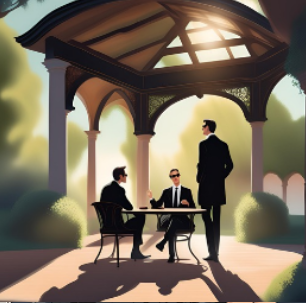
\includegraphics[width=5.88542in,height=5.79167in]{media/image4.png}

Der Morgen war kühl und neblig, als Julia, Martina und Michaels
Doppelgänger auf dem Campus der Universität Kassel ankamen. Ein
bleierner Dunst lag über den Gebäuden, und die angespannte Atmosphäre
war fast greifbar. Der Tag begann nicht wie jeder andere, und das
spürten sie bis in die Knochen. Bereits in der Ferne sahen sie die
ersten Protestschilder, die in den trüben Himmel gereckt wurden: „Gegen
Faschismus und Wissenschaftsfeinde!{\kern0pt}`` und „Weg mit dem
Reaktionär!{\kern0pt}`` hallte es von einer Gruppe Demonstranten, die
sich vor dem Hauptgebäude versammelt hatten.

„Das wird nicht leicht``, flüsterte Julia und sah sich mit besorgter
Miene um. Ihre Augen scannten die Menschenmenge, die in einem wütenden
Mosaik aus Gesichtern und Schildern zusammengepfercht war.

„Wir müssen uns beeilen``, sagte Michaels Doppelgänger und straffte die
Schultern, die wie ein Schild gegen die aufkommende Kälte standen. „Der
Professor wartet auf uns. Je schneller wir ihn von hier wegbringen,
desto geringer ist die Chance, dass sie uns erkennen.``

Martina nickte und warf einen prüfenden Blick auf die grauen Wolken, die
den Himmel bedeckten, als ob sie ein ungeschriebenes Omen
heraufbeschworen. „I.R.A.R.A.H hat alles vorbereitet. Lasst uns keine
Zeit verlieren.``

Sie schlüpften unauffällig in eines der Nebengebäude, ihre Schritte
hastig, aber kontrolliert. Das Geräusch der Proteste draußen wurde
lauter, doch im Inneren des Universitätsgebäudes war es still. Der
Kontrast fühlte sich surreal an. In dem spärlich eingerichteten Büro
fanden sie Dr. Tobias Neumann, der in aller Eile seine Sachen in eine
abgenutzte Ledertasche packte.

Er war ein Mann mittleren Alters, mit scharfen Gesichtszügen und einem
Ausdruck von Erschöpfung und Entschlossenheit in den Augen, die tief in
seinen Höhlen lagen wie zwei Schatten in einer dunklen Gasse.

Als das Team eintrat, sah er auf und atmete erleichtert aus. „Ich habe
auf euch gewartet``, sagte er und legte die Tasche ab. „Die Lage draußen
spitzt sich zu. Die Demonstranten sind heute besonders aggressiv.``
Seine Stimme war ein rauer Faden, der sich durch die angespannte Luft
zog.

„Wir haben alles vorbereitet``, sagte Michaels Doppelgänger ruhig und
holte einen braunen Franziskanerhabit aus seiner Tasche. „Hier ist dein
Ordenshabit. Sobald du ihn anziehst, bist du offiziell Bruder Timotheus
-- ein Franziskaner auf dem Weg in die USA.``

Martina reichte ihm einen gefälschten Personalausweis. „I.R.A.R.A.H hat
dafür gesorgt, dass du eine neue Identität hast. Dein Ordensname und
deine neue Existenz sind gesichert.`` Die Worte lagen schwer auf den
Schultern des Professors, der das Gewicht seiner Situation spürte.

Dr. Neumann starrte den Habit an, bevor er sich entschlossen
aufrichtete. „Das ist verrückt``, murmelte er, während er sich in die
braune Kutte hüllte. „Aber ich habe keine andere Wahl.``

Kaum war er fertig, führten sie ihn durch die leeren Flure des
Universitätsgebäudes nach draußen. Vor der Tür parkte ein unauffälliger
Lieferwagen, doch der Weg dorthin war nicht ohne Risiko. Die Proteste
vor der Universität waren lauter geworden, und die Menge schien
angesichts der bevorstehenden Vorlesung des Professors aufgeheizt.

„Wir müssen da durch``, sagte Julia, während sie einen prüfenden Blick
auf die Menge warf. „Sie dürfen nicht merken, dass du es bist. Wir haben
nur wenig Zeit.``

„Ich werde mit ihm vorausgehen``, sagte Michaels Doppelgänger
entschlossen. „Sie sollen glauben, wir sind eine Gruppe Franziskaner auf
Pilgerreise.``

Dr. Neumann schüttelte den Kopf, während sie sich langsam auf die Menge
zubewegten. „Es ist verrückt, was aus diesen Gruppen geworden ist``,
flüsterte er. „Früher waren sie intellektuell. Heute sind es bezahlte
Demonstranten aus den linken Kommunen, die nur dafür hier sind, Krawall
zu machen.``

Die Demonstranten bemerkten sie kaum, als sie sich durch die Menge
schoben. Einige riefen Beleidigungen, andere hoben ihre Schilder, doch
keiner schien sie zu erkennen. Doch dann, kurz bevor sie den Lieferwagen
erreichten, ertönte ein Ruf aus der Menge: „Das ist er! Der reaktionäre
Professor!{\kern0pt}``

Die Augen der Protestierenden richteten sich auf sie, und für einen
Moment schien es, als würde die Situation eskalieren. Der Puls der Menge
beschleunigte sich wie das Dröhnen eines sich nähernden Sturms. Doch
Michaels Doppelgänger schob Dr. Neumann schnell in den Lieferwagen. Mit
einem dumpfen Knall schloss sich die Tür, und sie fuhren los, während
wütende Rufe hinter ihnen erklangen.

Auf der Autobahn nach Frankfurt war es im Wagen ruhig, doch die
Anspannung war noch immer spürbar, wie ein Strick, der überdehnt wird.
Der Professor lehnte sich zurück und seufzte schwer, der Druck auf
seiner Brust schien kurzzeitig nachzulassen. „Früher waren Diskussionen
möglich``, sagte er nachdenklich. „Heute sehe ich nur noch Wut und
Ignoranz. Die Antifa war einmal eine intellektuelle Bewegung, doch jetzt
ist sie zu einem Instrument des Hasses geworden. Man bezahlt sie dafür,
die Andersdenkenden mundtot zu machen.``

„Sie haben kein Interesse mehr an Argumenten``, stimmte Martina zu. „Es
geht nur noch darum, den Gegner zu vernichten.``

„Es ist eine traurige Entwicklung``, fügte Michaels Doppelgänger hinzu.
„Aber in den USA wirst du eine neue Chance haben. Dort kannst du frei
sprechen, ohne von der Cancel Culture bedroht zu werden.``

Der Professor nickte, doch seine Gedanken schienen noch bei den
Ereignissen in Deutschland zu verweilen. „Es ist schwer zu glauben, wie
schnell sich die Dinge geändert haben. Wir haben unser kritisches Denken
an die Technologie abgegeben. Ich hoffe, in den USA noch etwas retten zu
können.``

Am Frankfurter Flughafen angekommen, führte das Team den Professor durch
die Sicherheitskontrollen. Jeder Schritt musste präzise geplant sein,
denn ein einziger Fehler konnte ihre gesamte Operation gefährden. Julia
warf einen Blick über die Schulter, als der Professor seine Papiere an
die Sicherheitsbeamten übergab. Es dauerte nur einen Moment, doch es
schien eine Ewigkeit, bis der Beamte ihn durchwinkte.

„Sobald du in den USA bist, bist du sicher``, sagte Julia und legte dem
Professor eine Hand auf die Schulter. „I.R.A.R.A.H wird sich um alles
Weitere kümmern.``

Dr. Neumann nickte, eine Spur von Dankbarkeit in seinen Augen. „Ohne
eure Hilfe wäre ich verloren gewesen``, sagte er leise. „Ich schulde
euch mein Leben.``

Sie sahen ihm nach, als er durch das Gate ging und der Flug nach Chicago
aufgerufen wurde. Ein letztes Mal warfen sie einen Blick auf den Mann,
den sie gerettet hatten, bevor er hinter den Glastüren verschwand.

In den USA angekommen, wurde der Professor von einem Mitglied der
franziskanischen Gemeinschaft abgeholt und zur Franciscan University of
Steubenville gebracht. Das Team begleitete ihn auf dem weiten Weg zur
Hochschule, deren ruhige und friedliche Atmosphäre im Kontrast zu den
chaotischen Zuständen in Deutschland stand. Die Bäume, die den Campus
umgaben, wirkten wie stille Wächter, die die neuen Ankömmlinge
beschützten.

„Willkommen, Bruder Timotheus``, begrüßte ihn einer der Brüder mit einem
warmen Lächeln. „Ihr Ruf ist Ihnen vorausgeeilt. Wir freuen uns, Sie in
unserer Gemeinschaft willkommen zu heißen.``

„Es wird mir eine Ehre sein``, erwiderte der Professor und nickte
leicht, das Gewicht seiner neuen Identität fühlte sich sowohl befreiend
als auch bedrückend an.

Am Tag nach seiner Ankunft hielt der Professor seine Antrittsvorlesung
vor einer versammelten Gruppe von Franziskanern und Studenten. Das Team
saß im hinteren Teil des Saals und hörte aufmerksam zu, wie der
Professor seine Worte sorgfältig wählte. Die Aula war erfüllt von einer
stillen Erwartung, die Luft schien zu vibrieren, als er sprach.

„In einer Zeit, in der der Mensch seine Mündigkeit an die Technologie
abgibt``, begann er, „müssen wir uns wieder auf die Werte der Aufklärung
und der Rationalität besinnen. Nicht die Technik wird uns retten,
sondern das kritische Denken. Wir müssen den Humanismus gegen die
postmodernen Strömungen verteidigen.``

Die Worte hallten im Raum wider, und für einen Moment schien es, als
hätten die scharfen Kanten der Welt draußen keine Macht mehr über sie.
Ein kollektives Nicken ging durch die Reihen, die Studenten schienen den
Funken der Hoffnung zu spüren, der in den Professoren steckte. Doch die
Realität konnte nicht lange ignoriert werden.

Nach der Vorlesung trafen sich Martina, Julia und Michaels Doppelgänger
mit einem I.R.A.R.A.H-Agenten in einem der Hinterzimmer der Hochschule.
Der Agent war ein schmaler Mann mit einem ernsten Ausdruck,

der ihnen gegenübersaß, während sie ihre Eindrücke von dem, was
geschehen war, teilten.

„Es war riskant``, sagte der Agent, seine Stimme war ruhig und
kontrolliert. „Aber wir haben Informationen, dass einige der
Demonstranten in Deutschland das Ziel haben, auch die Franziskanische
Gemeinschaft zu infiltrieren. Es könnte sein, dass sie auf Dr. Neumann
aus sind.``

„Was können wir tun?{\kern0pt}``, fragte Julia besorgt.

„Wir müssen die Sicherheit des Professors gewährleisten und die
Verbindung zur Community stärken. Er ist ein Ziel geworden. Die Frage
ist nicht, ob sie versuchen werden, ihn zu finden, sondern wann.``

„Das bedeutet, wir müssen die Verteidigung verstärken``, fügte Martina
hinzu. „Er ist nicht nur ein Professor. Er ist ein Symbol.``

Der Agent nickte. „In den nächsten Wochen wird es entscheidend sein,
unsere Kommunikation abzusichern und die Bewegungen in der Community im
Auge zu behalten. Es wird Zeit brauchen, um die Wellen zu glätten, die
die Ereignisse in Deutschland hierher bringen.``

Die nächsten Tage waren geprägt von intensiven Diskussionen über
Strategien zur Wahrung der Sicherheit des Professors. Währenddessen
spürte Dr. Neumann, wie er allmählich in seine neue Identität
hineinwuchs. Er stellte fest, dass er eine Stimme hatte, die in der
neuen Welt gehört werden wollte -- und die Möglichkeiten, die er hier
hatte, ermutigten ihn.

Einmal in der Woche hielt er Vorträge, und die Aula füllte sich mit
Studenten, die gespannt seinen Ideen lauschten. Immer wieder erinnerte
er sich an die Kälte der Demonstrationen in Deutschland, an die
Bedrohungen, die seinen Geist gefangen gehalten hatten, und an die
hitzigen Debatten, die nie zu einem Ergebnis führten. Hier war die
Diskussion wieder möglich, und die Herzen der Menschen waren bereit,
sich für die Ideen des Humanismus zu öffnen.

Eines Abends, nach einem besonders ermutigenden Vortrag, saß er mit
seinen neuen Brüdern am Tisch. „Ich hätte nie gedacht, dass ich einmal
so lebendig sein würde``, sagte er und hob sein Glas. „Auf die Freiheit
des Geistes!{\kern0pt}``

„Auf die Freiheit des Geistes!{\kern0pt}``, riefen die anderen im
Einklang, und ein Gefühl von Gemeinschaft erfüllte den Raum.

Dr. Neumann fühlte sich zum ersten Mal seit Langem frei, und als er in
die Gesichter seiner Brüder sah, wusste er, dass er in Sicherheit war.
Die Schatten der Vergangenheit schienen zu verblassen, während er den
neuen Weg beschritt, der vor ihm lag.

In dieser neuen Welt konnte er sein Wissen und seine Leidenschaft für
die Wahrheit teilen, ohne die Furcht vor Verfolgung. Der Mensch brauchte
keine Zensur mehr, sondern den Mut, sich für die Wahrheit einzusetzen.
Und während die Dunkelheit in Deutschland noch immer wütete, blühte die
Hoffnung in den Hallen der Franciscan University.

\section{Flucht über die Theiß}\label{flucht-uxfcber-die-theiuxdf}

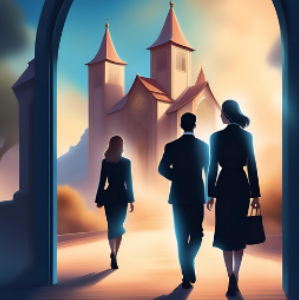
\includegraphics[width=6in,height=5.78125in]{media/image5.png}

Es war noch früh am Morgen, als sich das Team im Briefingraum der
Franziskanischen Hochschule in Steubenville versammelte. Die ersten
Sonnenstrahlen durchbrachen das Morgenlicht und tauchten den Raum in ein
sanftes Gold, doch die Atmosphäre war alles andere als entspannt. Ein
grelles Neonlicht flackerte über dem Tisch, der mit Unterlagen und
Notizen übersät war. Die Luft war gefüllt mit einer Mischung aus
Konzentration und Nervosität, während jeder Einzelne spürte, dass das,
was vor ihnen lag, weitreichende Konsequenzen haben könnte.

Dominierend an der Wand hing eine große Landkarte, auf der die geplante
Route durch Rumänien und entlang der Theiß in knallroter Farbe
eingezeichnet war. Die Kartenlinien schienen zu pulsieren, als würde die
Route selbst atmen, während das Team sich um den Tisch versammelte. Auf
einem großen Bildschirm flackerte die Zoom-Konferenz, in der die
Gesichter von ARS, Michael Phillips und Agent Novak zu sehen waren.

Agent Novak, der I.R.A.R.A.H-Einsatzleiter, war bereits vor der Kamera,
sein Blick fest und konzentriert. „Guten Morgen, alle zusammen``, begann
er, und seine Stimme strahlte sowohl Autorität als auch Besorgnis aus.
„Unsere Mission ist klar: Wir müssen zwei Männer sicher aus der Ukraine
bringen -- einen ukrainischen Pazifisten und einen russischen Deserteur.
Die Theiß ist die letzte Barriere, die wir überwinden müssen, bevor wir
nach Rumänien zurückkehren. Diese Region wird streng überwacht, und wir
haben nur ein kleines Zeitfenster.``

Ein murmelndes Raunen ging durch den Raum, als die Schwere der Aufgabe
sickerte. Jeder im Raum wusste, dass ihre Handlungen das Schicksal
dieser Männer in den Händen hielten. Die Kombination aus Angst und
Entschlossenheit lag spürbar in der Luft.

Der Bildschirm wechselte zu ARS, der künstlichen Intelligenz, die sie
als Unterstützung in dieser kritischen Mission hatten. Ihre beruhigende,
fast menschlich wirkende Stimme erfüllte den Raum: „Die Fluchtroute
wurde sorgfältig geplant. Wir haben die Positionen der Grenzpatrouillen
erfasst und den sichersten Punkt für die Überquerung der Theiß
ausgewählt. Die Kommunikation während der Mission wird über
verschlüsselte Kanäle erfolgen. Michael wird via Satellitentelefon
jederzeit in Kontakt bleiben.``

Michael Phillips, der als Teamleiter fungierte, nickte zustimmend. Seine
Augen strahlten eine Mischung aus Zuversicht und Besorgnis aus, als er
sich an sein Team wandte. „Denkt daran, das Leben dieser Männer liegt in
unseren Händen. Jeder falsche Schritt könnte bedeuten, dass wir
auffliegen. Also bleibt ruhig und konzentriert. Es ist wichtig, dass wir
als Team zusammenarbeiten.``

Er sah in die Gesichter seiner Kollegen und bemerkte die
Entschlossenheit, die sich in ihren Zügen widerspiegelte. Doch er konnte
auch die Unsicherheit wahrnehmen, die wie ein Schatten über dem Raum
schwebte. „Wir haben alles vorbereitet, und ich vertraue auf eure
Fähigkeiten. Wenn wir zusammenhalten und uns gegenseitig unterstützen,
können wir diese Herausforderung meistern.``

Ein kurzes Nicken, ein ermutigendes Lächeln hier und da, und die
Anspannung im Raum begann sich langsam zu lösen. Sie waren nicht allein
in diesem Kampf; jeder wusste, dass sie als Einheit stark waren, vereint
durch ein gemeinsames Ziel.

„Jetzt zu den Details``, fuhr Michael fort und wandte sich wieder der
Landkarte zu. „Wir werden uns in einem kleinen Dorf am Ufer der Theiß
treffen. Dort wartet der Kontaktmann auf uns, der uns zu den Männern
führen wird. Die Flucht muss schnell und leise verlaufen -- keine
Lichtsignale, keine Geräusche. Jeder von uns hat eine Rolle, und wir
müssen uns an den Plan halten. Fragen?{\kern0pt}``

Ein paar Hände hoben sich, und Michael beantwortete die Fragen mit
klaren, präzisen Antworten. Als er das letzte Wort sprach, spürte er,
dass das Team bereit war.

„Gut, wir haben wenig Zeit. Versammelt eure Ausrüstung und trefft euch
in einer halben Stunde im Garagenbereich. Jeder weiß, was zu tun ist.``

Das Team erhob sich, und als sie den Raum verließen, war die
Entschlossenheit in ihren Schritten spürbar. Michael blieb einen Moment
länger stehen, die Karte vor sich betrachtend. Die Linien, die in rot
gezeichnet waren, schienen wie ein Puls zu schlagen, und er konnte nicht
umhin, über die Verantwortung nachzudenken, die auf seinen Schultern
lastete.

„ARS``, murmelte er, und die künstliche Intelligenz antwortete prompt:
„Ja, Michael?{\kern0pt}``

„Gibt es Risiken, die wir übersehen haben könnten?{\kern0pt}``

„Alle relevanten Informationen sind in der Analyse enthalten. Die
Wahrscheinlichkeiten sind günstig, solange wir den festgelegten
Zeitrahmen einhalten und keine Abweichungen vom Plan vornehmen.``

Ein letztes tiefes Durchatmen, dann wandte Michael sich zum Gehen. Die
Herausforderung war groß, aber inmitten der Unsicherheiten schien ihm
die Möglichkeit, zwei Leben zu retten, die Mühe wert zu sein.

Die Mission war im Gange, und die Zeit tickte unbarmherzig. Sie mussten
sich beeilen, denn der Fluss der Theiß war nicht nur ein geographisches
Hindernis -- er war ein Symbol für Freiheit und Hoffnung, die sie in
dieser gefährlichen Welt suchten.

Das Team bestieg einen Flug von New York nach Bukarest, und die
Passagiere saßen angeschnallt in ihren Sitzen, während sich die Wolken
wie ein endloses Meer unter ihnen ausbreiteten. In der ersten Klasse, wo
das Team der I.R.A.R.A.H Platz genommen hatte, war die Atmosphäre von
einer gespannten Erwartung durchzogen. Captain Lukas Berger, ein
erfahrener Hochseekapitän mit einem tiefen Verständnis für die Gefahren
der Flucht, lehnte sich leicht vor und sprach mit einer Stimme, die
sowohl Respekt als auch Autorität ausstrahlte.

„Die Strömung auf der Theiß ist unberechenbar``, erklärte er mit einem
ernsten Blick, während er die Karte des Flusses studierte, die auf dem
Tisch lag. „Wir müssen schnell und leise sein. Der Motor des Boots ist
gedämpft, aber jede Bewegung kann Aufmerksamkeit erregen. Die Region
wird streng überwacht.``

Julia, die neben ihm saß, hörte aufmerksam zu. Ihr Blick war ernst, und
sie wusste, dass die Verantwortung, die sie trugen, nicht leicht zu
schultern war. „Jeder von uns muss seinen Teil perfekt erledigen. Unsere
Fehler dürfen nicht die Freiheit anderer gefährden``, entgegnete sie
bestimmt, während sie die Schwere ihrer Mission verinnerlichte.

In einer anderen Reihe unterhielten sich Michael Doppelgänger und Dr.
Neumann, der Professor, den sie zuvor in Sicherheit gebracht hatten.
Ihre Unterhaltung war leise, fast gedämpft, während sie über die
zunehmende Überwachung durch Technologie und die schleichende Erosion
der persönlichen Freiheit diskutierten. Dr. Neumann blickte nachdenklich
aus dem Fenster, als ob er die Wolken betrachten würde, die wie
unerfüllte Gedanken über der Erde schwebten. „Transhumanismus und Cancel
Culture gehen Hand in Hand``, murmelte er. „Sie versuchen, den Diskurs
durch Kontrolle zu ersticken, und Technik wird dabei als Werkzeug
benutzt.``

Michael Doppelgänger nickte energisch. „Deshalb müssen wir zeigen, dass
Freiheit etwas anderes ist als technologische Überlegenheit. Das ist die
Mission von I.R.A.R.A.H. Unsere Werte sind untrennbar mit der
menschlichen Würde verbunden.``

Nachdem sie in Bukarest gelandet waren, spürten sie den Druck der
bevorstehenden Aufgabe. Die Reise nach Sighetu Marmației, einer
Grenzstadt an der Theiß, war lang und ermüdend. Fast neun Stunden
dauerte die Fahrt, und während sie durch die malerischen, jedoch von den
Überresten vergangener Konflikte geprägten Landschaften rollten,
übernahm ARS die Kontrolle über die Kommunikation. „Ihr nähert euch dem
Fluss``, sagte die beruhigende Stimme von ARS über das verschlüsselte
Funkgerät. „Haltet euch an die geplante Route. Ich habe die
Patrouillenbewegungen in Echtzeit im Blick.``

Die Landschaft, die sie passierten, war melancholisch und doch schön,
mit weitläufigen Feldern und alten, verwitterten Dörfern, die
Geschichten von Hoffnung und Verzweiflung flüsterten. Als sie
schließlich am vereinbarten Ort ankamen, parkten sie das Fahrzeug an
einem abgelegenen, schattigen Platz, wo das dichte Unterholz sie vor den
neugierigen Blicken der Passanten schützte.

Der leise, beruhigende Klang des Flusses war in der Luft zu hören, als
sie sich zu Fuß durch das Dickicht bewegten. Mit jedem Schritt schien
die Anspannung zu wachsen. Schließlich entdeckten sie das Boot, das von
I.R.A.R.A.H bereitgestellt worden war, versteckt zwischen hohen Bäumen,
mit einem gedämpften Motor, der geduldig darauf wartete, gestartet zu
werden.

Der Himmel war von bedrohlichen, dunklen Wolken bedeckt, die wie ein
Vorbote ihrer Mission schienen. Als das Team in das Boot stieg und die
Motoren ansprangen, durchbrach ein Adrenalinstoß die angespannte Stille.
Captain Berger nahm das Steuer in die Hand und navigierte durch das
kalte, dunkle Wasser der Theiß. Die Strömung war stärker, als er
erwartet hatte, aber seine Erfahrung hielt ihn ruhig und konzentriert.
„Wir nähern uns dem Treffpunkt``, meldete ARS über das Funkgerät. „Die
Männer sind in einem Waldstück am ukrainischen Ufer versteckt. Wir haben
nur wenige Minuten, um sie zu finden.``

Die anderen starrten gebannt auf den Horizont, und als sie schließlich
die andere Seite des Flusses erreichten, sahen sie zwei Gestalten aus
dem Gebüsch hervortreten. Ihre Gesichter waren ein Bild der Erschöpfung
und der Nervosität, geprägt von Angst und Hoffnung. „Schnell, kommt an
Bord!{\kern0pt}``, rief Julia ihnen zu und half ihnen hastig ins Boot.
Kaum waren die Männer sicher an Bord, drängte Captain Berger das Boot
mit aller Kraft zurück zum rumänischen Ufer.

Plötzlich blitzte ein Lichtschein am Horizont auf -- eine Patrouille war
in der Ferne sichtbar. „Beeilt euch!{\kern0pt}``, rief Berger, und der
Motor des Boots heulte auf, als er den Gashebel nach vorn drückte. Das
Boot spritzte durch das Wasser, während Michael Doppelgänger einen
Stoffumhang über die Seite hielt, um sie vor den Scheinwerfern zu
verbergen. „Bleibt ruhig!{\kern0pt}``, flüsterte Julia, als sie die
Männer beobachtete, deren Anspannung greifbar war. „Es wird alles gut.
Wir sind auf dem richtigen Weg.``

Endlich erreichten sie das Ufer auf rumänischer Seite. Hastig zogen sie
das Boot ins Dickicht, und ein lokaler I.R.A.R.A.H-Kontakt wartete
bereits darauf, ihnen zu helfen, das Boot zu verstecken und später zu
entsorgen. „Wir werden es versenken, damit es keine Spuren gibt``,
erklärte der Kontakt leise, während seine Augen unruhig die Umgebung
scannten. „ARS hat uns einen sicheren Fluchtweg gezeigt. Aber wir müssen
uns beeilen. Die Patrouillen könnten jede Minute hier sein.``

Schnell halfen sie den geretteten Männern aus dem Boot und führten sie
durch das Dickicht zu einem kleinen, abgelegenen Jesuitenkloster, das
als Zufluchtsort für Flüchtlinge diente. Die Jesuiten hatten bereits
Vorkehrungen getroffen, um die Männer aufzunehmen und ihnen neue
Identitäten zu besorgen. Ein älterer Priester mit ruhigem Blick und
einem sanften Lächeln begrüßte sie. „Ihr habt viel riskiert, um diese
Männer hierher zu bringen``, sagte er mit einer Stimme, die sowohl Ruhe
als auch Trost ausstrahlte. „Sie sind nun in Sicherheit, und wir werden
uns um sie kümmern.``

Julia fühlte eine Welle der Erleichterung über sich hinwegziehen, als
sie sich von den Geretteten verabschiedete. „Es ist gut zu wissen, dass
sie hier Zuflucht gefunden haben``, flüsterte sie, während der Druck von
ihren Schultern abfiel und ihr Herz leichter wurde.

Nachdem sie die Geretteten in Sicherheit gebracht hatten, machte sich
das Team auf den Weg nach Ungarn. Sie wählten eine abgelegene Route über
die Grenze, um nicht entdeckt zu werden, und erreichten schließlich eine
kleine Stadt in Nordost-Ungarn, wo sie sich neu formieren konnten.
Michael kontaktierte Julia über das Satellitentelefon. „Ihr habt es
geschafft. I.R.A.R.A.H hat bestätigt, dass keine Hinweise auf eure
Anwesenheit zurückgeblieben sind. Gute Arbeit.``

„Danke``, antwortete Julia. „Aber wir wissen, dass dies erst der Anfang
ist.`` Die Mission war erfolgreich beendet, doch die nächsten
Herausforderungen warteten bereits.

Julia bereitete sich darauf vor, in Ungarn ihre Arbeit als
Sozialarbeiterin und psychologische Beraterin aufzunehmen, während
Martina in der Archäologie Fuß fassen wollte. Doch tief in ihnen wusste
jeder, dass die Zeit der Ruhe nur von kurzer Dauer sein würde. Die
Flucht über die Theiß war nur ein kleiner Sieg im Kampf gegen die
Unterdrückung, und die Wellen der Veränderung, die sie angestoßen
hatten, würden nicht aufhören.

In den kommenden Tagen, während sie sich in ihrem neuen Leben
einrichteten, wurden die Nachrichten über neue Repressionen in der
Ukraine und Russland immer drängender. Das Team war sich bewusst, dass
sie sich vorbereiten mussten. Agent Novak kontaktierte sie mit einer
neuen Anweisung. „Die Situation verschärft sich``, sagte er am Telefon,
und seine Stimme klang besorgt. „Wir haben Berichte über ein
bevorstehendes groß angelegtes Militärmanöver an der Grenze. Wir müssen
die Augen offenhalten und bereit sein, sofort zu handeln.``

„Das lässt uns keine Ruhe``, murmelte Julia, als sie das Telefon
auflegte. „Aber wir sind bereit. Immer bereit.``

Die gefährliche Mission an der Theiß war abgeschlossen, doch die Gefahr
war damit nicht vorbei. Ihre Reise hatte sie stärker gemacht, und die
Entschlossenheit in ihren Herzen brannte heller denn je. Gemeinsam
würden sie die nächste Mission annehmen, die I.R.A.R.A.H ihnen
anvertraute, egal wie herausfordernd sie auch sein mochte.

\section{Wiedersehen in Budapest}\label{wiedersehen-in-budapest}

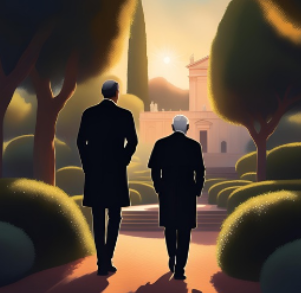
\includegraphics[width=6in,height=5.58333in]{media/image1.png}

Die kühle Morgenluft umhüllte Michael, als er vor dem Eingang des
Kollegium Germanicum in Rom stand. Der steinerne Bau mit seinen alten
Mauern schien ihn stumm zu verabschieden. Er spürte das Gewicht der
Jahre, die er hier verbracht hatte, und die Erinnerungen, die in den
Wänden gespeichert waren. Die Sonne brach durch die Wolken und tauchte
die Fassaden in ein sanftes, goldenes Licht. Mit einem letzten Blick auf
die vertraute Umgebung ließ er die schwere Holztür hinter sich zufallen.

Draußen wartete Maria auf ihn, in einen leichten Mantel gehüllt, der
sanft im Morgenwind flatterte. Ihr Blick war ruhig, doch in ihren Augen
lag ein Ausdruck, der Michael für einen Moment innehalten ließ. Es war
der Blick einer Frau, die viel zu sagen hatte, aber die Worte in der
Stille gefangen hielt.

„Also, es ist soweit``, sagte sie, ihre Stimme weich, aber durchzogen
von einer Melancholie, die die Luft um sie herum schwer machte. „Du
reist ab und lässt alles hinter dir.``

Michael nickte langsam. „Ja, es ist Zeit. Es gibt viel zu tun in
Budapest.`` Er hielt kurz inne und sah ihr tief in die Augen. „Ich
hoffe, du weißt, dass ich immer noch an dich denke\ldots{} und an alles,
was wir geteilt haben.``

Ein leichtes Lächeln huschte über Marias Lippen, doch ihre Augen
verrieten eine tiefere Geschichte. „Pass auf dich auf, Michael. Es ist
gut zu wissen, dass du die Familie nicht vergisst.``

Für einen Augenblick schien es, als läge in ihren Worten mehr, als sie
aussprach. Michael wusste, dass die Andeutung über die Vergangenheit und
die Identität des Doppelgängers wie ein unausgesprochener Schatten
zwischen ihnen stand. Er neigte den Kopf, und ohne ein weiteres Wort
wandte er sich ab, um zum Taxi zu gehen, das ihn zum Flughafen bringen
würde.

Der Flug nach Budapest verlief ruhig. Während er durch das Fenster auf
die unter ihm vorbeiziehende Landschaft blickte, kreisten seine Gedanken
um das, was vor ihm lag -- und was er in Rom zurückgelassen hatte. Der
Gedanke an Maria, an die unausgesprochenen Worte, die zwischen ihnen
schwebten, drängte sich in den Vordergrund. Als das Flugzeug auf dem
Flughafen Budapest landete, durchzog ein vertrautes Kribbeln der
Vorfreude seinen Körper. Es war nicht nur eine neue Aufgabe, die auf ihn
wartete, sondern auch die Möglichkeit, endlich Klarheit zu schaffen.

Ein schwarzer Wagen wartete auf ihn. Die Fahrt durch die Stadt führte
ihn vorbei an der Donau und den prächtigen Gebäuden, die im goldenen
Abendlicht erstrahlten. Das Wasser funkelte in der Dämmerung und schien
die Vergangenheit und Zukunft zu reflektieren, während er auf dem Weg zu
der kleinen Wohnung war, die Julia und Martina mittlerweile ihr Zuhause
nannten. Sie hatten sich gut eingelebt und schienen in Budapest eine
neue Bestimmung gefunden zu haben.

Als der Wagen vor dem alten Gebäude hielt, atmete Michael tief durch.
Alte Bäume umrahmten den Eingang, und die vertrauten Klänge der Stadt
erfüllten die Luft. Er drückte die Klingel und wartete, während seine
Gedanken weiter um die unausgesprochene Wahrheit kreisten, die ihn
hierher geführt hatte.

Die Tür öffnete sich, und Martina begrüßte ihn mit einem warmen Lächeln,
das ein Stück der Anspannung von seinen Schultern nahm. „Michael, schön,
dich zu sehen. Komm rein, wir haben auf dich gewartet.``

Im Wohnzimmer herrschte eine heimelige Atmosphäre. Der Duft von frisch
gebrühtem Kaffee erfüllte den Raum, und auf dem Couchtisch standen
Kuchen und Gebäck bereit, die wie kleine Kunstwerke aussahen. Julia kam
aus der Küche, ein Tablett in den Händen, das sie mit einem strahlenden
Lächeln absetzte. „Endlich bist du da``, sagte sie und sah Michael mit
einem Ausdruck der Erleichterung an. „Setz dich, nimm dir einen Kaffee.
Wir haben viel zu besprechen.``

Michael nahm Platz auf einem der alten Sofas, die mit einem liebevollen,
aber abgewetzten Stoff bezogen waren. Die Gemütlichkeit des Raumes gab
ihm ein Gefühl von Heimat, das er lange vermisst hatte. Kurz darauf
betrat auch der Doppelgänger den Raum. Er wirkte entspannt, aber auch
ein wenig nervös, als er Michael gegenüber Platz nahm. „Willkommen in
Budapest``, sagte er mit einem leichten Lächeln, das sowohl Offenheit
als auch Unsicherheit verriet. „Es ist schön, die ganze
\textquotesingle Familie\textquotesingle{} beisammen zu haben.``

Das Wort „Familie`` klang für Michael ungewohnt vertraut, und der
Ausdruck im Gesicht des Doppelgängers schien für einen kurzen Moment
eine tiefere Verbundenheit zu verraten. Michael erwiderte das Lächeln,
während ihm ein Gedanke durch den Kopf schoss -- war es wirklich
möglich, dass dieser junge Mann sein Sohn war?

„Danke``, sagte Michael und nahm einen Schluck von seinem Kaffee, der
warm und aromatisch war. „Es fühlt sich gut an, hier zu sein.``

Sie plauderten über Belangloses -- die Stadt, die Arbeit und das Leben
in Budapest. Doch zwischen den Gesprächen schwebte eine ungesprochene
Frage im Raum, eine Spannung, die weder Julia noch Martina zu lösen
schienen. Der Doppelgänger warf Michael hin und wieder Blicke zu, die
von einem intensiven Interesse durchdrungen waren, als ob er eine
Bestätigung suchte, die Michael noch nicht ausgesprochen hatte.

Das Abendessen verlief entspannt. Die Gespräche waren leicht und voller
Lachen, doch als sie sich schließlich in der Dämmerung auf dem Balkon
niederließen, lag über der Szene eine Art von stiller Verständigung.
Michael wusste, dass es an der Zeit war, Antworten zu suchen -- und dass
er sie möglicherweise bereits vor sich hatte.

„Manchmal``, begann er leise, als die ersten Sterne am Himmel
aufleuchteten, „führt uns das Leben auf unerwartete Wege, die wir erst
später verstehen.`` Er sah den Doppelgänger an und bemerkte, dass dieser
seine Worte aufmerksam verfolgte. „Und manchmal treffen wir Menschen,
die uns zeigen, dass es mehr Verbindungen gibt, als wir zunächst
glauben.``

Die Nacht senkte sich über Budapest, und die Lichter der Stadt blinkten
wie kleine Funken, die Erinnerungen in die Dunkelheit warfen. Die
Blicke, die sie tauschten, sprachen Bände, während die Stille des Abends
sie umgab. Michael wusste, dass es Zeit brauchen würde, um die Wahrheit
vollständig auszusprechen, aber in diesem Moment genügte es, dass sie
zusammen waren.

Die Familie hatte eine neue Dimension bekommen -- eine, die er zwar
nicht erwartet, aber vielleicht immer erhofft hatte. Und während das
sanfte Rauschen der Donau in der Ferne zu hören war, wusste Michael,
dass dies erst der Anfang einer langen und spannenden Reise war.

\end{document}
